%\pagenumbering{arabic}
%\setcounter{page}{1}


\section{Dirt Spot Sweeping Random Strategy}

Dirt Spot Sweeping Random (DSSR) strategy is a new random test strategy developed during this study. DSSR strategy is the combination of two existing strategies i.e. pure random and random plus with the addition of one new strategy called spot sweeping. It is based on two intuitions. Intuition No. 1 is that boundaries have interesting values and using these values in isolation can provide high impact on test results, while intuition No. 2 is that faults can reside in block and strip pattern thus using neighbouring values of the fault finding value can lead us to the next fault in the same block or strip. This increases the performance of the test strategy in terms of executing fewer number of test cases with more number of faults. It is to be noted that random plus test strategy add border values before the test starts whereas spot sweeping test strategy add fault finding values and its neighbouring values to the list of interesting values at run time when they are found during testing.\\

Initially, the DSSR strategy was not utilizing the boundary values of random plus strategy and the list of interesting values was empty at the start of the test. Therefore, in the earlier version, the test had to start with random testing and once the fault was found in the system, DSSR strategy would transfer the fault finding test value and the surrounding values to the list of interesting values. In this way the list of interesting values is populated and the strategy now looks for interesting values in the list before trying to get any arbitrary random value. The bottle-neck in this strategy was that DSSR strategy had to wait for the random testing to find the fault in the system. This bottle-neck was removed by introducing border values in DSSR strategy while keeping the remaining process the same. In updated version the border values are added to the list of interesting values before the test starts thus from the beginning of the test the system not only selects purely random values but also checks for values from boundary values, which increases the fault finding chances and consequently add more values to the list of interesting values \cite{Kaner2004}.\\

\begin{figure}[htp]
\centering
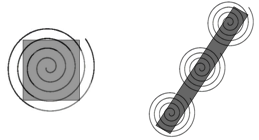
\includegraphics[width=8cm,height=3cm]{figures/block2.png}
\caption{DSSR covering block and strip pattern}
\label{fig:block2}
\end{figure}

Figure \ref{fig:block2} shows how DSSR strategy explores the faults residing in the block and strip patterns of a program. The testing process starts with pure random and random plus strategy. When the fault is found the DSSR strategy adds the value whose input causes the fault and its neighbouring values to the list of interesting values. Now if that fault is positioned on the point pattern then the added values will work to find new faults but if the fault is positioned on the block or strip pattern then the neighbouring values will explore the whole block and strip pattern by finding new faults and adding its neighbours values untill all the faults in that block or strip are identified. The faults coverage from the block and strip pattern is shown in spiral form because first fault will lead to second, second to third and will continue untill it ends.\\

Before its implementation and evaluation, the following research questions about the DSSR strategy were formulated and subsequently addressed:\\
\begin{enumerate}

\item To get highly efficient algorithm to cope with the combination of strategies including pure random, random plus containing border values and spot sweeping which further populate the list of interesting values with fault finding value and its neighbouring values to provide more relevant test values to the Test engine. \\

\item To get high number of unique faults because according to Chen et al. \cite{Chen2006} most of the faults reside in block and strip pattern which is efficiently covered by DSSR strategy. \\

\item To get  low number of unique faults and high number of similar faults because the faults in the same block and strip pattern across the program might be of similar nature.\\

\item  Not to get any particular improvement if the program don't contain any block or strip pattern but contain only point pattern.\\

\item  DSSR strategy might consume more time to execute the same set of test cases than random and random plus strategy because of extra processing when analyzing values at runtime and transferring them to the list of interesting values.\\



\end{enumerate}

\subsection{Structure of Dirt Spot Sweeping Random Strategy}

\hspace{10 mm}The DSSR strategy is explained with the help of flow-chart in Figure \ref{fig:Working_DSSS}. In this process the DSSR strategy continuously track the number of faults during the exection of the test session. This tracking is done in an efficient way with 0 or minimum overhead \cite{Leitner2009}. Execution of test is performed normally untill a fault is found in the SUT. When a fault is found the program not only copy the value that lead to the fault, but also copy its surrounding values to the variable list of interesting values. From the flow-chart you can see that if the fault finding value is of primitive type then the test strategy DSSR finds the type of that primitive value and add values only of that particular type to the interesting values list. Addition of these values increases the size of the list of interesting values which provide relevant test data for the remaining test session and the new generated test cases are more targeted towards finding new faults in the given SUT.\\

\begin{figure}[htp]
\centering
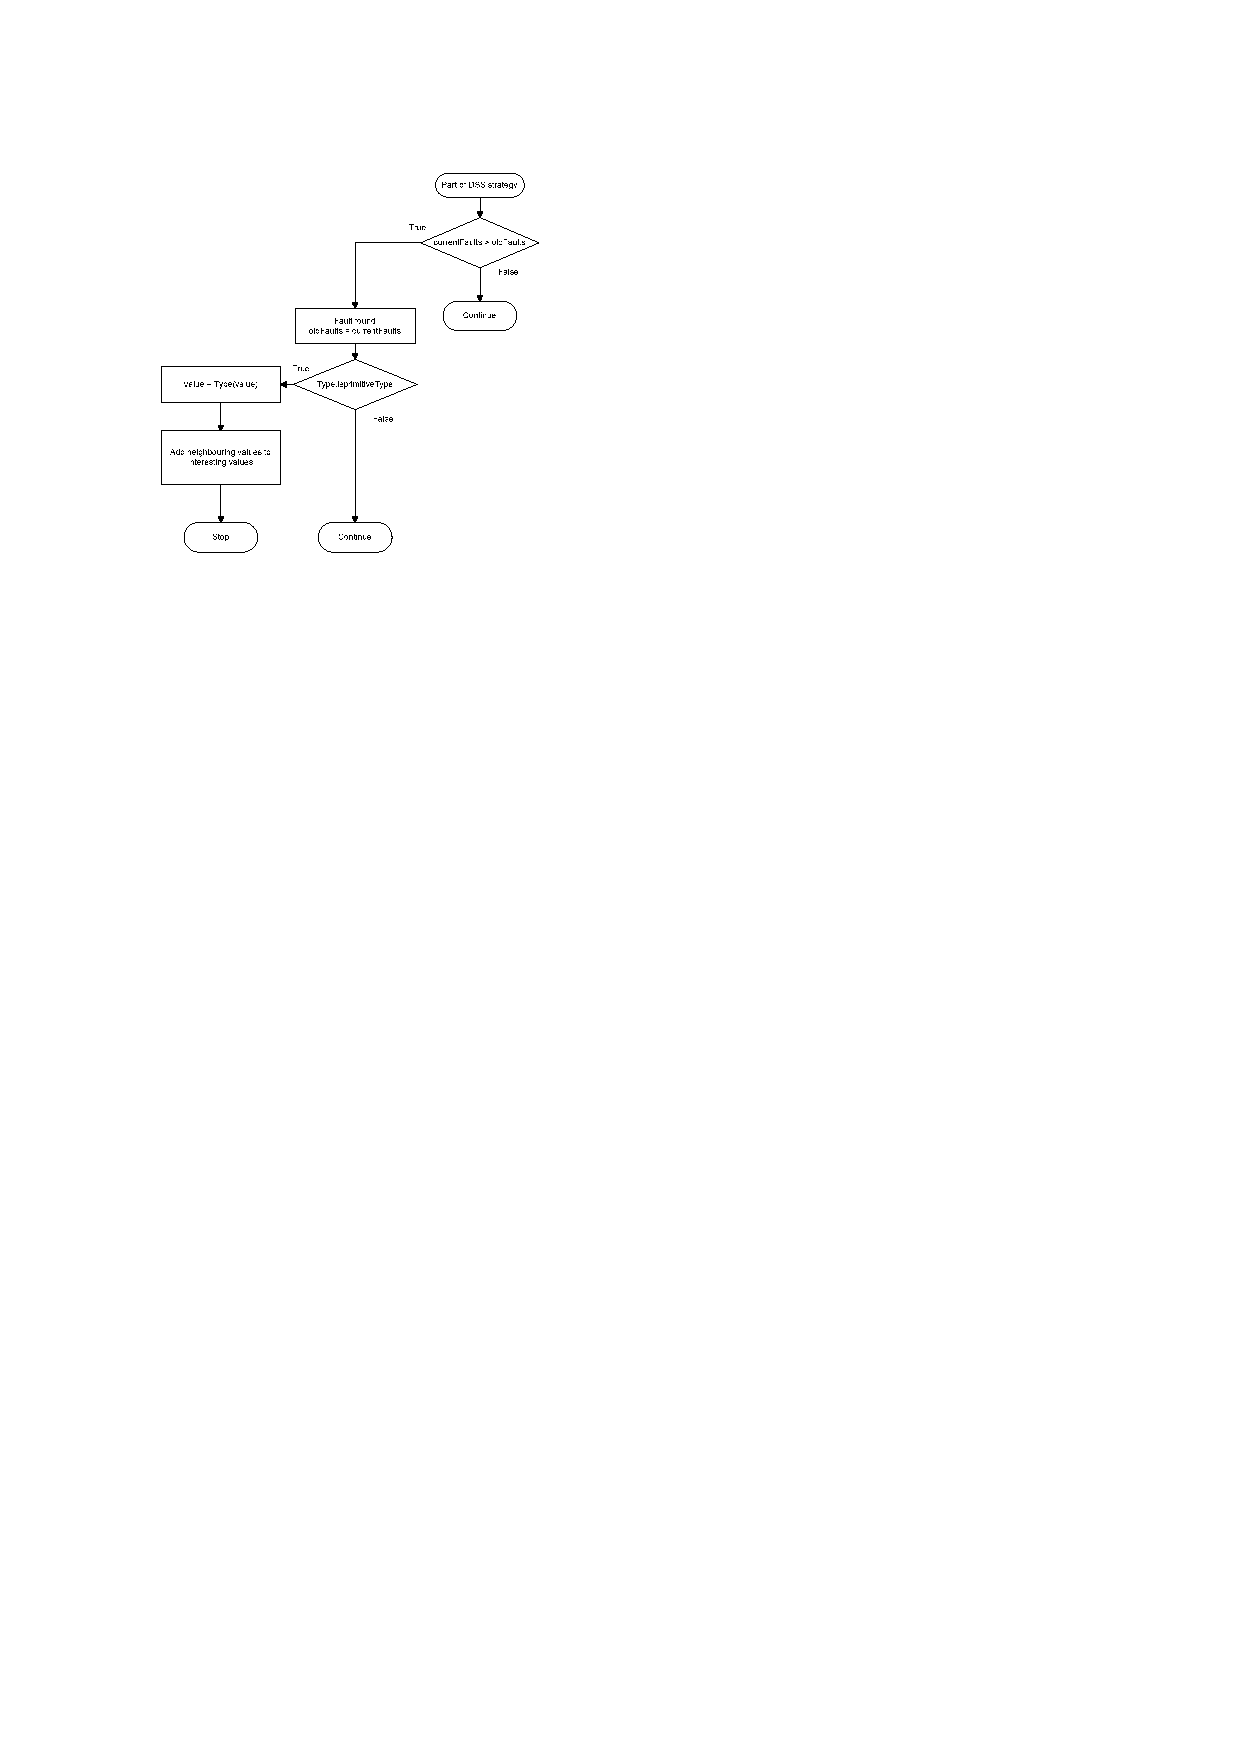
\includegraphics[width=8.5cm,height=12cm]{figures/flowchart1.pdf}
\caption{Working mechanism of DSSR Strategy}
\label{fig:Working_DSSS}
\end{figure}

Border values and other special fault finding values are added to the list by random plus strategy (extention of pure random) prior to the start of test session where as to sweep the failure pattern, fault value and fault surrounding values are added at run time after a fault is found. Table \ref{table:addvalues} contains the values that are added to the list of interesting values when a fault is found. The test value is represented by X where X can be int, double, float, long, byte, short, char and String. All values are converted to their respective types before adding to the list of interesting values.

\begin{table}[ht]
\scriptsize
\caption{Neighbouring values for primitive types and String} % title of Table
\centering % used for centering table
\begin{tabular}{| l | l |} % centered columns (4 columns)
\hline\hline %inserts double horizontal lines
Type & Values to be added\\ [0.5ex] % inserts table
%heading
\hline % inserts single horizontal line
\multirow{3}{*}{X is int, double, float, long, byte short and char} & X \\ % inserting body of the table

&[[X-3 , X-1]] \\
&[[X+1 , X+3]]\\
\hline
\multirow{8}{*}{X is String} & X\\ % inserting body of the table

& X + ``  "\\ % inserting body of the table
& ``  " + X \\ % inserting body of the table
& X.toUpperCase() \\
& X.toLowerCase() \\
& X.trim() \\
& X.substring(2) \\
& X.substring(1, X.length() - 1) \\[1ex]
\hline
\hline %inserts single line
\end{tabular}
\label{table:addvalues} % is used to refer this table in the text
\end{table}


\subsection{Motivating Example}
% no \IEEEPARstart
To further clarify the working mechanism of DSSR strategy we have written the following simple program which is planted with atleast three faults. The first one is division by zero exception while the other two are in the form of assertion statements at line 3 and 4.  Below we describe how DSSR strategy will perform execution when the following class is supplied for testing.\\



public class Math \{\\

\hspace{7mm} public void calc ( int a) \{\\

//Square the value and assign it to result.\\*

1.\hspace{12mm} int result1 = a * a;\\*

2. \hspace{12mm}int result2 = result1 / a;\\*

//To check that the value of result is positive.\\*

3.\hspace{12mm} assert result1 $>$ a;\\*

//To check that the revert of result is the received value.\\*

4. \hspace{12mm}assert Math.sqrt(result1) = a;\\*



\hspace{7mm}\}  \\*

\}\\*

\hspace{10 mm}From the above code we can see that only one primitive type is used which is ``int" and we also know that for ``int" beside other values we have special pre-defined values including 0, Integer.MAX\_VALUE and Integer.MIN\_VALUE in the list of interesting values. Now on starting the test we will immediately find all the faults in the following order using DSSR strategy where as pure random strategy on the other hand will try randomly to find each fault although the faults are laying very close to each other.\\*



\textbf{Fault 1:} The DSSR strategy might select value 0 for variable ``a"  in the first test case because 0 is available in the list of interesting values and therefore its priority for selection is higher than other values. This will cause Java to generate division by zero from line 2 because any integer divided by zero is infinity.\\*

\textbf{Fault 2:} When DSSR strategy caught the failure it will add this and the surrounding values to the list of interesting values which includes 0, 1, 2, 3 and -1, -2, -3. Now for the second test case DSSR strategy may pick -3 as a test value and it will take us to our second fault where assertion no 2 (line 4) will fail because the square root of -3 will be +3 instead of the origina suppliedl number -3.\\*

\textbf{Fault 3:} After a few test cases the DSSR strategy might select Integer.MAX\_VALUE for variable ``a" which is also available in the list of interesting values and it will lead us to our 3rd fault because result1 will not be able to store the square of Integer.MAX\_VALUE. Instead of the actual calculated square value Java will assign a negative value (Java language rule) to variable result1 which will lead to the violation of assertion 1 (line 3) and we will get our 3rd and final fault.\\*


From the above execution process we can understand that, in this example, pre-defined values including border values, fault finding values and its surrounding values lead us quickly to the available faults and in less number of tests as compared to pure random which randomly selects test values across the whole input domain in a traditional fashion.

\section{Implementation of DSSR strategy}

The DSSR strategy was implemented in YETI tool \cite{Oriol2011}. YETI is an automated random testing tool developed in Java. It is an open source tool capable of testing both procedural and object-oriented softwares. Its language-agnostic meta model enables it to test programs written in multiple languages including Java, C\#, JML and .Net. The core features of YETI includes easy extensibility for future growth, speed of up to one million calls per minute on java code, real time logging, real time GUI support, ability to test programs using multiple strategies and auto generation of test report at the end of the test session. A number of hitherto faults have successfully been found by YETI in various production softwares. \\

YETI can be divided into three main sections including core infrastructure, language-specific bindings and strategies. The core infrastructure represents routines, a group of types and a pool of specific type objects. The  language specific bindings contain the code to make the call and process the results. The strategies section defines the way to select the class/module to test random selection of routine/method from the given module and get instances of the required type during testing. DSSR strategy is also added to the strategies section of YETI tool with the class name YetiDSSRStrategy. It is extention of YetiRandomStrategy which in itself is extention of an abstract class YetiStrategy. The class hierarchy is shown in Figure \ref{fig:hierarchyofDSSR}.\\

\begin{figure}[htp]
\centering
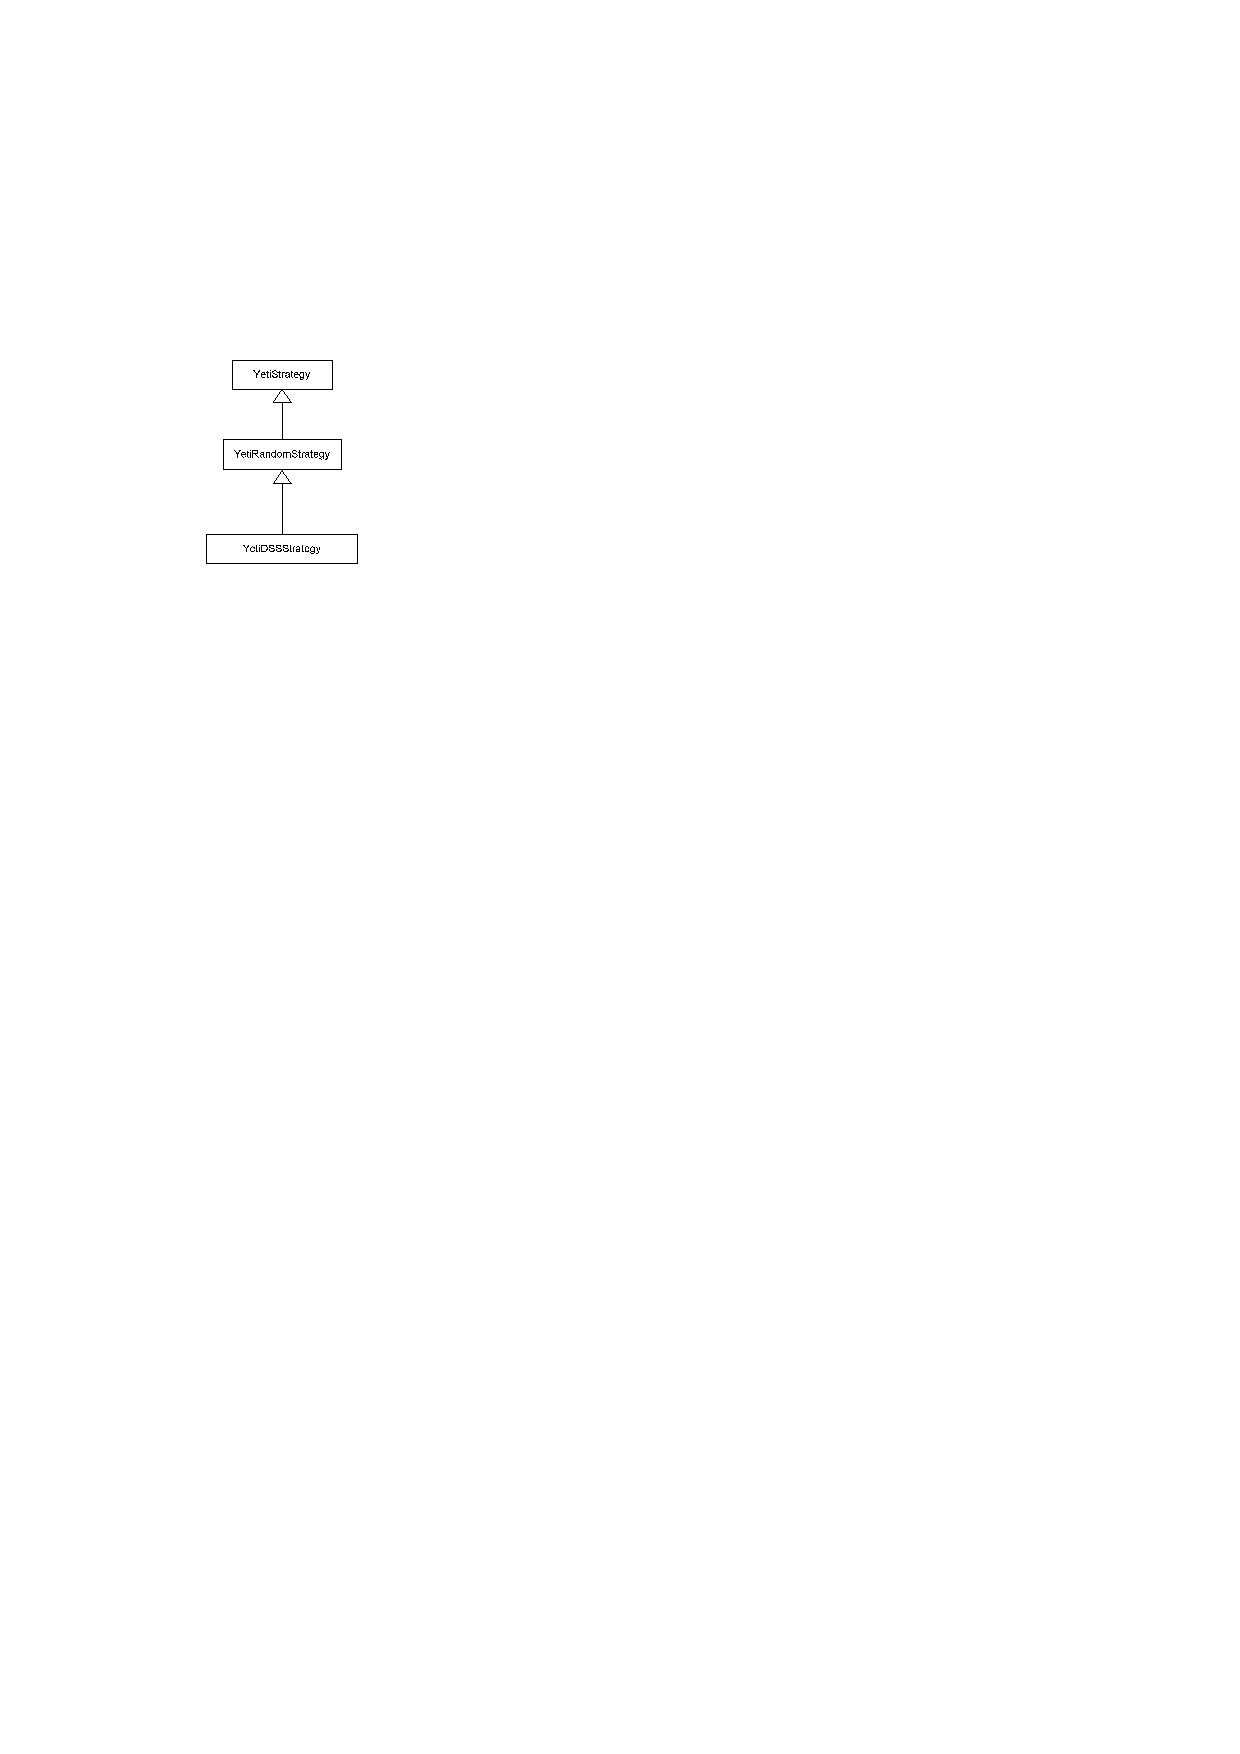
\includegraphics[width=5cm,height=7cm]{figures/hierarchy.pdf}
\caption{Class Hierarchy of DSSR in YETI}
\label{fig:hierarchyofDSSR}
\end{figure}


If no particular strategy is defined during test initialization then YETI will use its default random strategy in which the user can control the probability of null values and the percentage of newly created objects. Both probabilities are set to 10\% by default. \\

YETI also provide an interactive Graphical User Interface (GUI) where a user can see the progress of the current test in real time. Besides GUI, YETI also provides extensive logs of the test session which are very helpful in fault tracking. For more details about YETI see references \cite{Oriol2010a} and \cite{Oriol2010}.